\newpage
\chapter{TINJAUAN PUSTAKA} \label{Bab II}

\section{Tinjauan Pustaka} \label{II.Tinjauan}
Penelitian terkait teleskop robotik dan \textit{Mahony Filter} telah dilakukan oleh berbagai peneliti dengan pendekatan dan tujuan yang beragam. Beberapa studi fokus pada pengembangan perangkat keras, sistem kontrol otomatis, serta integrasi perangkat lunak untuk observasi langit secara efisien dan akurat. Tabel~\ref{table:2.literasi} merangkum beberapa penelitian yang relevan dan menjadi dasar dalam pengembangan sistem pada tugas akhir ini. \par
\begin{longtable}{| b{0.05\textwidth}|p{0.2\textwidth}|p{0.2\textwidth}|p{0.2\textwidth}|p{0.2\textwidth}|} % Longtable berguna agar tabel dapat terpotong di halaman baru
	\caption{Literasi Penelitian Terdahulu}
	\label{table:2.literasi}\\
	\hline
	\textbf{No.} & \textbf{Judul} & \textbf{Masalah} & \textbf{Metode} & \textbf{Hasil} \\
	\hline
	\endfirsthead % Header tabel untuk halaman pertama
	\hline
	\textbf{No.} & \textbf{Judul} & \textbf{Masalah} & \textbf{Metode} & \textbf{Hasil} \\
	\hline
	\endhead % Header tabel untuk halaman selanjutnya (repeat header row)
	1.  & RUKYATUL HILAL INSTRUMENT DESIGN BASED ON ARDUINO  & Keterbatasan instrumen tradisional dalam pengamatan Hilal serta penempatan bulan yang tidak konsisten & \textit{Reasearch \& Development} (R\&D) & Hasil penelitian menunjukkan bahwa instrumen berbasis Arduino berhasil menunjukkan posisi lebih tepat ke Bulan. \cite{Hadi2022}.\\ 
	\hline
	2. & Design and Development of Real-Time Controller Based on ARM Cortex-M Processor
	for Automated Altitude-Azimuth Telescope Mount & Observasi astronomi manual menghadapi beberapa tantangan signifikan seperti mengarahkan teleskop secara manual dan kondisi cuaca yang tidak menentu & Nested Vectored Interrupt Controller (NVIC) terintegrasi, dan Digital Signal Processing (DSP) engine & Hasil penelitian menunjukkan bahwa pengontrol STM32 F407VGT6 berbasis mikrokontroler berhasil dikembangkan dan diuji, serta memenuhi persyaratan yang ditetapkan \cite{Rangana2022}.\\ 
	\hline
	3. & Characterization of the Small Robotic Telescope Instrument and Implementation at ITERA Lampung Astronomical Observatory & keterbatasan metode manual, kesulitan dalam mengarahkan teleskop secara presisi, dan masalah kontras untuk objek redup seperti bulan tetap, serta artefak noise pada kamera & In-situ test observations & OZT-ALTS berhasil melakukan pengamatan bulan tetap dengan kontras yang lebih baik dan mampu mendeteksi exoplanet yang transit \cite{Malasan2025}.\\ 
%Teleskop robotik 36~cm dengan kamera sCMOS dan software berbasis ZeroMQ serta PSO untuk penjadwalan otomatis.
	\hline
	4. & Sistem Pelacak Otomatis Gerakan Benda Langit Pada Teleskop Refraktor Berbasis Mikrokontroler & Saat ini teleskop yang tersedia sebagian besar hanya dapat melakukan pelacakan gerak bintang saja. & Reasearch \& Development (R\&D) & Hasil penelitian menunjukkan bahwa sistem yang
	dibangun dapat melakukan pelacakan secara otomatis pergerakan benda-benda langit dengan akurat. \cite{Burhanuddin2014}.\\
	\hline
	5. & Indirect tuning of a complementary orientation filter using velocity data and a genetic algorithm & bagaimana meningkatkan akurasi pelacakan posisi menggunakan IMU berbiaya rendah di lingkungan tanpa GNSS & \textit{Popular Baseline Filter} \& \textit{Time Agnostic Velocity Error} & Metode \textit{Mahony Filter} menunjukkan kinerja lebih baik dibandingkan \textit{Madgwick Filter} dan Q-EKF, dengan nilai kesalahan kecepatan (\textit{MSVE} dan \textit{WRVE}) yang lebih rendah \cite{Maton2024}.\\ 
	\hline
\end{longtable}
Dari  penelitian yang ditinjau dari Table~\ref{table:2.literasi}, terlihat adanya perkembangan signifikan pada instrumen astronomi, mulai dari desain berbasis Arduino untuk rukyatul hilal, sistem kontrol real-time berbasis \textit{ARM Cortex-M}, hingga teleskop robotik kecil yang mampu mendeteksi eksoplanet. Penelitian-penelitian tersebut menunjukkan arah pengembangan menuju otomatisasi dan peningkatan akurasi pengamatan benda langit.

Namun, terdapat beberapa kesenjangan penelitian (\textit{research gap}), yaitu:

\begin{enumerate}[noitemsep]
	\item Sebagian besar penelitian masih berfokus pada pengendalian teleskop atau peningkatan kualitas pengamatan, tetapi belum banyak yang mengintegrasikan metode optimasi sensor IMU untuk estimasi orientasi dan posisi.
	
	\item Tantangan terkait akurasinya sensor berbiaya rendah.
	
	\item Penerapan algoritma cerdas seperti \textit{Genetic Algorithm} (GA) dan \textit{Fuzzy Inference System} (FIS) pada filter komplementer masih relatif baru dan menunjukkan potensi besar untuk meningkatkan performa sistem teleskop robotik.
	
\end{enumerate}

Dengan demikian, penelitian ini menjadi relevan karena menawarkan pendekatan penyempurnaan estimasi sudut teleskop berbasis IMU yang dioptimalkan dengan \textit{Mahony Filter} guna meningkatkan estimasi sudut dan posisi, sehingga diharapkan dapat mengatasi keterbatasan pada penelitian sebelumnya dan meningkatkan presisi teleskop \textit{Alt-Azimuth} otomatis.

\section{Dasar Teori} \label{II.Teori}
Pada bagian ini akan dibahas teori-teori dasar yang menjadi landasan dalam perancangan dan pengembangan sistem teleskop robotik \textit{Alt-Azimuth} dengan estimasi sudut menggunakan \textit{Mahony Filter}. Pembahasan mencakup konsep dasar teleskop robotik, sistem koordinat \textit{Alt-Azimuth}, sensor inersial, serta algoritma \textit{Mahony Filter} sebagai metode optimasi estimasi sudut. Teori-teori ini menjadi acuan dalam proses perancangan perangkat keras dan perangkat lunak pada penelitian ini. \par
\subsection{Teleskop} \label{II.Teori1}
Teleskop adalah alat optik yang digunakan untuk mengamati objek yang sangat jauh, seperti Bintang, planet dan benda-benda Antariksa lainnya\cite{Bradley2014}. Alat ini bekerja dengan cara mengumpulkan dan memfokuskan cahaya sehingga menghasilkan citra yang tampak lebih besar \cite{Bradley2014} \cite{HannuKarttunen2017} \cite{Roy2018}. \par

Dalam perkembangannya, teleskop kini banyak dikembangkan menjadi sistem otomatis atau robotik yang dapat beroperasi tanpa campur tangan manusia \cite{Dyer2020}. Teleskop robotik mampu mengikuti pergerakan benda langit secara kontinu, memudahkan pengamatan jangka panjang, pelacakan objek cepat, serta memungkinkan pengendalian jarak jauh melalui jaringan internet atau lokal. \par

\begin{enumerate}[noitemsep]
	\item Dapat dibuat dengan ukuran yang jauh lebih besar.
	
	\item Bebas aberasi kromatik, karena cahaya dipantulkan, bukan dibiaskan.
	
	\item Cocok untuk pengamatan objek redup, seperti nebula atau galaksi.
\end{enumerate}

Namun demikian, kelemahan dari teleskop reflektor adalah lebih rentan terhadap penyimpangan optik akibat kesalahan kolimasi (penyelarasan cermin), serta permukaan cermin yang memerlukan perawatan khusus agar tetap bersih dan reflektif. \par

\subsection{Trigonometri Bola} \label{II.Teori2}

Ketika kita menghubungkan 3 buah lingkaran pada sebuah bola kita akan menemukan segitiga yang terbentuk dari lingkaran yang berpotongan tersebut seperti yang ditunjukin pada Gambar~\ref{fig:2.2}, Segitiga ini dinamakan segitiga bola\cite{Roy2018}. 
\begin{figure}[H] % Kalau menggunakan H, posisi gambar akan tepat dibawah teks
	\centering
	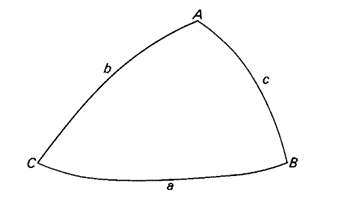
\includegraphics[width=0.6\textwidth]{figure/segitiga_bola.png}
	\caption{Segitiga Bola}
	\label{fig:2.2}
	{\footnotesize Sumber: Astronomy Principles and Practice} % Untuk memberikan sumber
\end{figure}
Trigonometri bidang atau trigonometri pada umumnya dapat digunakan untuk menghitung / merumuskan persamaan yang dapat digunakan untuk menghitung sejumlah properti yang ada di segitiga bola. Ada banyak persamaan yang dihasilkan, akan tetapi 4 rumus khusus yang lebih sering digunakan dari pada rumus lainnya yang ditunjukan oleh \ref{eq:2.formulaSinus} hingga \ref{eq:2.formulaEmpatBagian} \cite{Roy2018}.
\begin{enumerate}[noitemsep]
	\item Formula sinus
	\begin{equationcaptioned}[eq:2.formulaSinus]{
			\frac{\sin{A}}{\sin{a}} = \frac{\sin{B}}{\sin{b}} = \frac{\sin{C}}{\sin{c}}
		} {
		Formula sinus trigonometri bola
		}
	\end{equationcaptioned}
	\item Formula cosinus
	\begin{equationcaptioned}[eq:2.formulaCosinus]{
			\begin{split}
				\cos{a} = \cos{b} \cos{c} + \sin{b} \sin{c} \cos{A}\\
				\cos{b} = \cos{a} \cos{c} + \sin{a} \sin{c} \cos{B}\\
				\cos{c} = \cos{a} \cos{b} + \sin{a} \sin{b} \cos{C}
			\end{split}
		} {
			Formula cosinus trigonometri bola
		}
	\end{equationcaptioned}
	\item Formula analogi cosinus
	\begin{equationcaptioned}[eq:2.formulaAnalogiCosinus]{
			\sin{a}\sin{B} = \cos{b}\sin{c} - \sin{b}\cos{c}\cos{A}
		} {
			Formula analogin cosinus
		}
	\end{equationcaptioned}
	\item Formula 4 bagian
	\begin{equationcaptioned}[eq:2.formulaEmpatBagian]{
			\cos{a}\cos{C} = \sin{a}\cot{b} - \sin{C}\cot{B}
		} {
			Formula 4 bagian
		}
	\end{equationcaptioned}
\end{enumerate}
\subsection{\textit{Julian Date}} \label{II.Teori3}
\textit{Julian Date} (JD) merupakan sistem penanggalan yang digunakan secara luas dalam astronomi untuk menyatakan waktu dalam bentuk bilangan real yang menyatakan jumlah hari (dan pecahannya) sejak tengah hari (12:00 UT) pada tanggal 1 Januari 4713 SM dalam kalender Julian. Sistem ini diperkenalkan untuk menghindari kompleksitas kalender masehi seperti tahun kabisat dan perbedaan bulan, serta untuk menyederhanakan perhitungan selisih waktu antara dua peristiwa astronomis\cite{HannuKarttunen2017}. Julian date pada tanggal tertentu dapat dihitung dengan \ref{eq:2.julianDate} \cite{HannuKarttunen2017}
\begin{equationcaptioned}[eq:2.julianDate]{
		J = 367y - \left\lfloor \frac{7(y + \frac{m + 9}{12})}{4} \right\rfloor - \left\lfloor \frac{3 \left( \left\lfloor \frac{y + \frac{m - 9}{7}}{100} \right\rfloor + 1 \right)}{4} \right\rfloor + \left\lfloor \frac{275m}{9} \right\rfloor + d + s	
	}{
		Julian Date
	}
\end{equationcaptioned}
\begin{equationcaptioned}[eq:2.julianDateKoreksi]{
		s = 1721029 + \frac{h}{24} + \frac{m}{60} + \frac{s}{3600}	
	}{
		Koreksi Waktu Julian Date
	}
\end{equationcaptioned}

Dengan:
\begin{description}[noitemsep]
	\item[$J$] = Nilai \textit{Julian Date}.
	\item[$y$] = Tahun (\textit{year}).
	\item[$m$] = Bulan (\textit{month}).
	\item[$d$] = Hari (\textit{day}).
	\item[$h$] = Jam dalam format 24 jam (\textit{hour}).
	\item[$M$] = Menit (\textit{minute}).
	\item[$s$] = Detik (\textit{second}).
	\item[$\lfloor \cdot \rfloor$] Fungsi lantai (\textit{floor}), yaitu pembulatan ke bawah.
\end{description}

\subsection{\textit{Local Sidereal Time}} \label{II.TeoriLST}

Waktu sideris (\textit{Sidereal Time}) merupakan ukuran waktu astronomi yang didasarkan pada rotasi Bumi relatif terhadap bintang-bintang jauh, bukan terhadap Matahari seperti pada waktu matahari rata-rata. Satu hari sideris memiliki durasi sekitar 23 jam 56 menit, sedikit lebih pendek dibandingkan satu hari matahari \cite{Meeus1998}. 

Waktu sideris lokal (\textit{Local Sidereal Time}, LST) menyatakan posisi titik vernal ($\Upsilon$) relatif terhadap meridian pengamat dan digunakan secara langsung dalam penentuan sudut jam (\textit{Hour Angle}) suatu objek langit. LST dapat dihitung dari waktu sideris Greenwich (\textit{Greenwich Sidereal Time}, GST) dengan menambahkan bujur geografis pengamat sebagai berikut \cite{Meeus1998}:

\begin{equationcaptioned}[eq:2.lst]{
		LST = GST + \lambda
	}{
		Perhitungan Local Sidereal Time
	}
\end{equationcaptioned}

dengan:
\begin{description}[noitemsep]
	\item[$LST$] = Waktu sideris lokal (derajat).
	\item[$GST$] = Waktu sideris Greenwich (derajat).
	\item[$\lambda$] = Bujur geografis pengamat (positif ke arah timur).
\end{description}

Dalam sistem teleskop robotik, nilai LST digunakan untuk mengonversi koordinat ekuatorial ke koordinat horizontal (Alt-Azimuth) secara real-time agar teleskop dapat mengikuti pergerakan objek langit akibat rotasi Bumi.


\subsection{Tata Koordinat Langit} \label{II.Teori4}
Tata koordinat langit adalah sistem referensi dua dimensi yang digunakan untuk menentukan posisi benda langit di bola langit, yaitu proyeksi imajiner langit malam sebagai bola yang mengelilingi Bumi \cite{Roy2018} \cite{HannuKarttunen2017} \cite{Bradley2014}. Sistem ini analog dengan sistem koordinat geografis di Bumi (lintang dan bujur), namun diproyeksikan ke langit. Tata koordinat langit dibagi menjadi beberapa sistem utama yang digunakan tergantung pada kebutuhan dan titik referensinya.
\subsubsection{Tata Koordinat Azimuth} \label{II.Teori4.1}


Tata Koordinat Azitmuth merupakan tata koordinat paling primitif dan merupakan yang paling mudah untuk dibayangkan. Tata koordinat ini memanfaatkan sudut azimuth (A) yang dihitung dari utara kearah timur dengan rentang sudut 0° sampai 360° dan altitude (a) yang dihitung dari horizon ke zenith pengamat dengan rentang sudut -90° sampai 90°\cite{Roy2018} seperti yang ditunjukkan pada Gambar~\ref{fig:2.3}. 
\begin{figure}[H] % Kalau menggunakan H, posisi gambar akan tepat dibawah teks
	\centering
	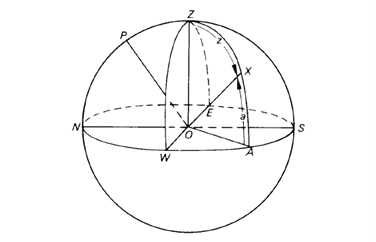
\includegraphics[width=0.6\textwidth]{figure/tata_koordinat_azimuth.png}
	\caption{Tata koordinat azimuth}
	\label{fig:2.3}
	{\footnotesize Sumber: Astronomy Principles and Practice} % Untuk memberikan sumber
\end{figure}
Ada beberapa titik istimewa di tata koordinat azimuth. Seperti Zenith merupakan titik yang berada tepat di atas kepala pengamat dan Nadir yang merupakan titik berada di bawah pengamat. Kekurangan dari tata koordinat ini adalah koordinat yang bergantung dengan lokasi pengamat sehingga tidak cocok digunakan sebagai acuan katalog.

\subsubsection{Tata Koordinat Ekuatorial} \label{II.Teori4.2}

Tata koordinat ekuator adalah sistem koordinat langit yang digunakan untuk menentukan posisi benda-benda langit secara global dan tidak bergantung pada lokasi atau waktu pengamatan di Bumi \cite{Roy2018}. 
\begin{figure}[H] % Kalau menggunakan H, posisi gambar akan tepat dibawah teks
	\centering
	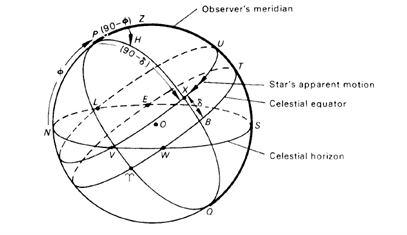
\includegraphics[width=0.6\textwidth]{figure/tata_koordinat_ekuatorial.png}
	\caption{Tata koordinat ekuatorial}
	\label{fig:2.4}
	{\footnotesize Sumber: Astronomy Principles and Practice} % Untuk memberikan sumber
\end{figure}
Berdasarkan Gambar~\ref{fig:2.4}, Sistem ini menggunakan dua parameter utama: Right Ascension ($\alpha$), dihitung dari titik $\Upsilon$ sampai titik B dan dinyatakan dalam satuan jam (0h hingga 24h), serta Declination ($\delta$), yang setara dengan garis lintang dan dinyatakan dalam derajat (-90° hingga +90°) relatif terhadap ekuator langit\cite{Roy2018} seperti yang ditunjukin pada Gambar~\ref{fig:2.4}. Karena posisinya tetap terhadap bintang-bintang jauh, sistem ini sangat ideal untuk katalog astronomi dan digunakan secara luas dalam pengoperasian teleskop otomatis.
\subsubsection{Tata Koordinat Ekliptika} \label{II.Teori4.3}

Tata koordinat ekliptika adalah sistem koordinat langit yang beracuan pada bidang ekliptika, yaitu bidang lintasan semu Matahari terhadap bola langit akibat revolusi Bumi mengelilingi Matahari \cite{Roy2018}. Sistem koordinat ini sangat berguna dalam kajian dinamika tata surya karena posisi Matahari, planet, dan benda-benda minor banyak dinyatakan relatif terhadap bidang ekliptika. 

\begin{figure}[H]
	\centering
	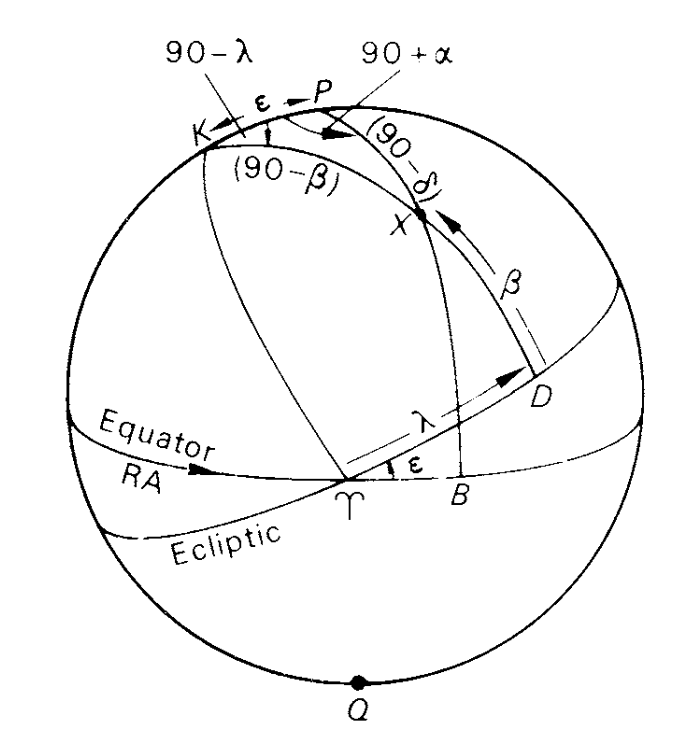
\includegraphics[width=0.6\textwidth]{figure/tata_koordinat_ekliptika.png}
	\caption{Tata koordinat ekliptika}
	\label{fig:2.5}
	{\footnotesize Sumber: Astronomy Principles and Practice}
\end{figure}

Berdasarkan Gambar~\ref{fig:2.5}, sistem koordinat ekliptika menggunakan dua parameter utama: bujur ekliptika ($\lambda$), yang diukur sepanjang bidang ekliptika dari titik vernal (titik $\Upsilon$) ke arah timur, dengan rentang 0° hingga 360°, dan lintang ekliptika ($\beta$), yaitu sudut suatu benda langit terhadap bidang ekliptika dengan rentang -90° hingga +90° \cite{Roy2018}. Karena didefinisikan terhadap bidang ekliptika, sistem koordinat ini sangat sesuai untuk menggambarkan orbit benda-benda tata surya dan analisis gerak planet serta komet.

\subsubsection{Transformasi Tata Koordinat Equatorial ke Azimuth} \label{II.Teori4.32}
\begin{figure}[H] % Kalau menggunakan H, posisi gambar akan tepat dibawah teks
	\centering
	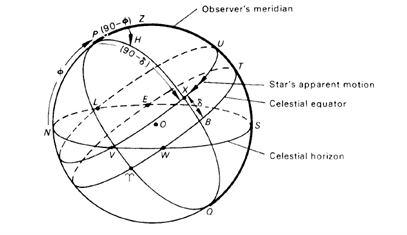
\includegraphics[width=0.6\textwidth]{figure/tata_koordinat_ekuatorial.png}
	\caption{Tata koordinat ekuatorial}
	\label{fig:2.5}
	{\footnotesize Sumber: Astronomy Principles and Practice} % Untuk memberikan sumber
\end{figure}
Transformasi koordinat dari sistem ekuator (Right Ascension dan Declination) ke sistem alt-azimuth (Azimuth dan Altitude) diperlukan agar teleskop dapat mengarahkan diri ke posisi objek langit berdasarkan lokasi dan waktu pengamatan\cite{Roy2018}. Berdasarkan gambar \ref{fig:2.5} dapat kita rumuskan.
\begin{equationcaptioned}[eq:2.transformasiDeklinasi]{
			\sin{\delta} = \sin{\phi}\sin{a} + \cos{\phi}\cos{a}\cos{A}
	} {
		Transformasi koordinat nilai deklinasi
	}
\end{equationcaptioned}
\begin{equationcaptioned}[eq:2.transformasiAltitudo]{
		\sin{a} = \sin{\phi}\sin{\delta} + \cos{\phi}\cos{\delta}\cos{H}
	} {
		Transformasi koordinat nilai altitudo
	}
\end{equationcaptioned}
\begin{equationcaptioned}[eq:2.transformasiHA1]{
		\cos{H} = \frac{\sin{a}-\sin{\phi}\sin{\delta}}{\cos{\phi}\cos{\delta}}
	} {
		Transformasi koordinat Hour Angle 1
	}
\end{equationcaptioned}
	\begin{equationcaptioned}[eq:2.transformasiHA2]{
			\tan{H} = \frac{\sin{A}}{\sin{\phi}\cos{A}-\cos{\phi}\tan{a}}
		} {
			Transformasi koordinat Hour Angle 2
		}
	\end{equationcaptioned}
Dengan:
\begin{description}[noitemsep]
	\item[$\delta$] = Deklinasi objek.
	\item[$\phi$] = Lintang pengamat.
	\item[$a$] = \textit{Altitude} (ketinggian) objek.
	\item[$A$] = \textit{Azimuth} objek.
	\item[$H$] = \textit{Hour Angle} atau sudut jam yang dihitung dari horizon pengamat ke zenit.

\end{description}
\subsubsection{Transformasi Tata Koordinat Ekliptika ke Ekuatorial} \label{II.Teori4.33}

\begin{figure}[H]
	\centering
	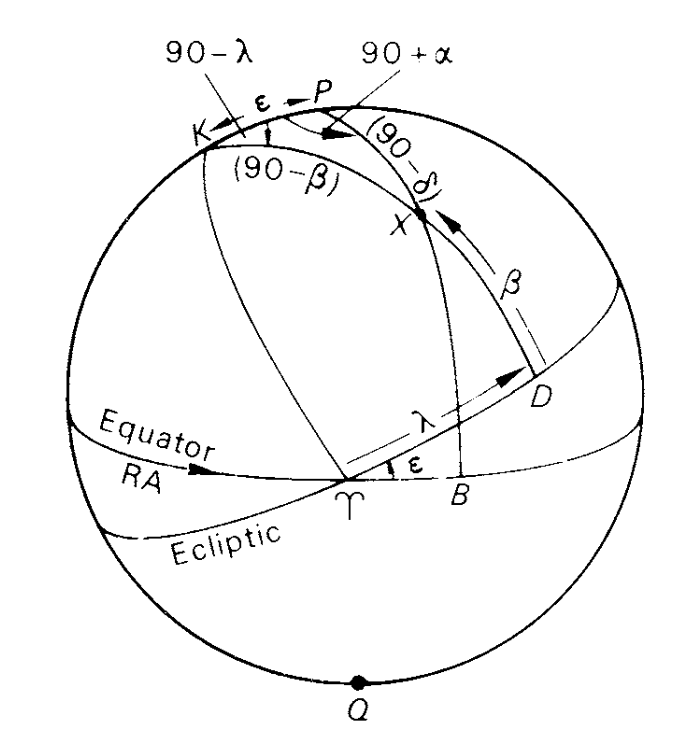
\includegraphics[width=0.6\textwidth]{figure/tata_koordinat_ekliptika.png}
	\caption{Tata koordinat ekliptika}
	\label{fig:2.7}
	{\footnotesize Sumber: Astronomy Principles and Practice}
\end{figure}

Transformasi koordinat dari sistem ekliptika (bujur ekliptika $\lambda$ dan lintang ekliptika $\beta$) ke sistem ekuatorial (Right Ascension $\alpha$ dan Declination $\delta$) diperlukan karena data orbit benda-benda tata surya umumnya dinyatakan dalam koordinat ekliptika, sedangkan teleskop otomatis bekerja dalam koordinat ekuatorial \cite{Roy2018}. Transformasi ini dipengaruhi oleh sudut kemiringan Bumi terhadap bidang ekliptika yang dikenal sebagai sudut eksentrisitas ($\varepsilon$).

Besarnya eksentrisitas rata-rata adalah
{\setlength{\abovedisplayskip}{8pt}%
	\setlength{\belowdisplayskip}{8pt}%
	\[
	\begin{split}
\varepsilon \approx 23^{\circ}.44
	\end{split}
	\]}


Hubungan transformasi koordinatnya dinyatakan sebagai berikut.

\begin{equationcaptioned}[eq:2.transformasiDekEklKeEku]{
		\sin{\delta} = \sin{\beta}\cos{\varepsilon} + \cos{\beta}\sin{\varepsilon}\sin{\lambda}
	}{
		Transformasi lintang ekliptika ke deklinasi
	}
\end{equationcaptioned}

\begin{equationcaptioned}[eq:2.transformasiRAcos]{
		\cos{\alpha}\cos{\delta} = \cos{\beta}\cos{\lambda}
	}{
		Transformasi komponen kosinus Right Ascension
	}
\end{equationcaptioned}

\begin{equationcaptioned}[eq:2.transformasiRAsin]{
		\sin{\alpha}\cos{\delta} = 
		\cos{\beta}\sin{\lambda}\cos{\varepsilon} - \sin{\beta}\sin{\varepsilon}
	}{
		Transformasi komponen sinus Right Ascension
	}
\end{equationcaptioned}

Right Ascension ($\alpha$) diperoleh dengan fungsi $\arctan2$ untuk menjaga kuadran sudut:

\begin{equationcaptioned}[eq:2.transformasiRAakhir]{
		\alpha = \arctan2
		\left(
		\cos{\beta}\sin{\lambda}\cos{\varepsilon} - \sin{\beta}\sin{\varepsilon},
		\cos{\beta}\cos{\lambda}
		\right)
	}{
		Perhitungan Right Ascension dari koordinat ekliptika
	}
\end{equationcaptioned}

Sedangkan nilai deklinasi ($\delta$) diperoleh:

\begin{equationcaptioned}[eq:2.transformasiDekFinal]{
		\delta = \arcsin
		\left(
		\sin{\beta}\cos{\varepsilon} + \cos{\beta}\sin{\varepsilon}\sin{\lambda}
		\right)
	}{
		Perhitungan Declination dari koordinat ekliptika
	}
\end{equationcaptioned}

Dengan:
\begin{description}[noitemsep]
	\item[$\lambda$] = bujur ekliptika objek.
	\item[$\beta$] = lintang ekliptika objek.
	\item[$\alpha$] = Right Ascension objek.
	\item[$\delta$] = Declination objek.
	\item[$\varepsilon$] = sudut eksentrisitas Bumi (kemiringan sumbu Bumi).
\end{description}

Transformasi ini digunakan secara luas dalam mekanika benda langit karena posisi planet, komet, dan asteroid biasanya dinyatakan dalam sistem ekliptika, sedangkan pengamatan teleskop dan katalog bintang menggunakan sistem ekuatorial \cite{Roy2018}.

\subsection{\textit{Elemen Orbit Keplerian}} \label{II.TeoriElemenOrbit}

Elemen orbit Keplerian merupakan parameter-parameter yang digunakan untuk mendeskripsikan bentuk, orientasi, dan posisi benda langit pada lintasannya. Dengan enam buah elemen orbit, keadaan orbit planet atau satelit dapat ditentukan secara lengkap dalam model dua-benda \cite{Meeus1998}.

Elemen orbit Keplerian terdiri dari:

\begin{enumerate}
	\item \textbf{Sumbu semi-mayor ($a$)}\\
	Menunjukkan ukuran orbit elips, yaitu setengah jarak sumbu mayor.
	
	\item \textbf{Eksentrisitas ($e$)}\\
	Menentukan bentuk orbit. Nilai $e = 0$ menyatakan lingkaran sempurna, sedangkan $0 < e < 1$ menyatakan elips.
	
	\item \textbf{Inklinasi ($i$)}\\
	Merupakan sudut antara bidang orbit dengan bidang acuan, umumnya bidang ekliptika.
	
	\item \textbf{Bujur node naik ($\Omega$)}\\
	Merupakan sudut dari sumbu referensi menuju node naik (titik potong orbit saat benda bergerak dari selatan ke utara bidang acuan).
	
	\item \textbf{Argumen perihelion ($\omega$)}\\
	Merupakan sudut dari node naik menuju titik perihelion sepanjang lintasan orbit.
	
	\item \textbf{Mean anomaly ($M$)}\\
	Merupakan sudut fiktif yang menyatakan posisi benda langit sepanjang orbit sebagai fungsi waktu.
\end{enumerate}

Keenam elemen tersebut membentuk vektor elemen orbit sebagai berikut:

\begin{equationcaptioned}[eq:2.vektorElemenOrbit]{
		\mathbf{X} =
		(a, e, i, \Omega, \omega, M)
	}{
		Vektor elemen orbit Keplerian \cite{vallado}
	}
\end{equationcaptioned}

Elemen orbit digunakan sebagai dasar perhitungan posisi planet dalam koordinat kartesius maupun koordinat astronomis lain seperti koordinat ekliptika dan ekuatorial.

\subsection{\textit{Anomali Orbit}} \label{II.TeoriAnomali}

Anomali orbit adalah sudut-sudut yang digunakan untuk menyatakan posisi benda langit pada orbit elips. Terdapat tiga jenis anomali yang umum digunakan, yaitu mean anomaly, eccentric anomaly, dan true anomaly. Ketiganya saling berhubungan dan digunakan dalam perhitungan posisi orbit \cite{Meeus1998}.

\begin{enumerate}
	\item \textbf{Mean Anomaly ($M$)}\\
	Mean anomaly didefinisikan sebagai sudut fiktif yang bertambah secara linear terhadap waktu:
	
	\begin{equationcaptioned}[eq:2.meanAnomaly]{
			M(t) = M_{0} + n(t - t_{0})
		}{
			Mean anomaly sebagai fungsi waktu \cite{Meeus1998}
		}
	\end{equationcaptioned}
	
	dengan $n$ adalah \textit{mean motion} yang diberikan oleh:
	
	\begin{equationcaptioned}[eq:2.meanMotion]{
			n=\sqrt{\frac{\mu}{a^{3}}}
		}{
			Mean motion orbit \cite{vallado}
		}
	\end{equationcaptioned}
	
	\item \textbf{Eccentric Anomaly ($E$)}\\
	Eccentric anomaly merupakan sudut bantu pada lingkaran bantu elips yang digunakan dalam persamaan Kepler.
	
	\item \textbf{True Anomaly ($\nu$)}\\
	True anomaly adalah sudut antara vektor posisi benda langit dan perihelion, diukur dari fokus elips tempat Matahari berada.
	
	Hubungan antara eccentric anomaly ($E$) dan true anomaly ($\nu$) diberikan oleh persamaan:
	
	\begin{equationcaptioned}[eq:2.trueAnomaly]{
			\tan\left(\frac{\nu}{2}\right)
			=
			\sqrt{\frac{1+e}{1-e}}
			\tan\left(\frac{E}{2}\right)
		}{
			Hubungan antara eccentric anomaly dan true anomaly \cite{Meeus1998}
		}
	\end{equationcaptioned}
\end{enumerate}

Anomali orbit memungkinkan perubahan posisi benda langit direpresentasikan secara matematis dalam bentuk yang mudah dihitung secara numerik.


\subsection{\textit{Persamaan Kepler}} \label{II.TeoriPersamaanKepler}

Persamaan Kepler merupakan hubungan antara mean anomaly ($M$) dan eccentric anomaly ($E$) pada orbit elips. Persamaan ini menjadi inti dari perhitungan posisi benda langit terhadap waktu \cite{Meeus1998}.

Persamaan Kepler dituliskan sebagai:

\begin{equationcaptioned}[eq:2.persamaanKepler]{
		M = E - e\sin E
	}{
		Persamaan Kepler untuk orbit elips \cite{Meeus1998}
	}
\end{equationcaptioned}

Persamaan ini bersifat non-linear dan tidak memiliki solusi analitik tertutup sehingga perlu diselesaikan melalui metode numerik. Salah satu metode yang umum digunakan adalah metode Newton–Raphson, dengan formulasi iterasi sebagai berikut:

\begin{equationcaptioned}[eq:2.newtonKepler]{
		E_{k+1}
		=
		E_k
		-
		\frac{E_k - e\sin E_k - M}{1 - e\cos E_k}
	}{
		Metode Newton–Raphson untuk menyelesaikan persamaan Kepler \cite{vallado}
	}
\end{equationcaptioned}

Setelah nilai $E$ diperoleh, true anomaly ($\nu$) dapat dihitung melalui  \ref{eq:2.trueAnomaly}

Persamaan Kepler menjadi dasar dalam penentuan posisi planet, satelit buatan, serta sistem navigasi modern karena menghubungkan waktu dengan posisi benda langit pada orbitnya.

\subsection{Perhitungan Posisi Matahari} \label{II.TeoriMatahari}

Perhitungan posisi Matahari diperlukan dalam sistem teleskop robotik untuk keperluan observasi Matahari maupun pembatasan arah gerak teleskop demi keamanan instrumen. Posisi Matahari dapat ditentukan berdasarkan parameter orbit elips Bumi dengan pendekatan anomali rata-rata dan koreksi pusat (\textit{equation of center}) \cite{Meeus1998}. 

Bujur ekliptika Matahari ($\lambda$) dihitung dari bujur rata-rata dan koreksi anomali, kemudian ditransformasikan ke koordinat ekuatorial menggunakan sudut kemiringan ekliptika. Nilai Right Ascension ($\alpha$) dan Declination ($\delta$) Matahari diperoleh melalui transformasi koordinat ekliptika ke ekuatorial sebagaimana dijelaskan pada Subbab~\ref{II.Teori4.33}.

Pendekatan ini menghasilkan akurasi yang memadai untuk keperluan penunjukan (\textit{pointing}) dan pelacakan (\textit{tracking}) teleskop robotik \cite{Meeus1998}.
\subsection{Perhitungan Posisi Planet} \label{II.TeoriPlanet}

Posisi planet dihitung berdasarkan elemen orbit Keplerian dengan asumsi model dua-benda antara Matahari dan planet yang bersangkutan. Elemen orbit yang digunakan meliputi sumbu semi-mayor, eksentrisitas, inklinasi, bujur node naik, argumen perihelion, dan anomali rata-rata \cite{Meeus1998,EMStandish1992}. 

Melalui penyelesaian persamaan Kepler, diperoleh nilai anomali eksentrik dan anomali sejati yang selanjutnya digunakan untuk menentukan posisi planet dalam koordinat heliosentris. Koordinat tersebut kemudian ditransformasikan ke sistem ekliptika dan ekuatorial agar dapat digunakan oleh sistem teleskop otomatis. Pendekatan ini umum digunakan pada sistem teleskop robotik dengan kebutuhan akurasi menengah \cite{meeus}.

\subsection{Perhitungan Posisi Bulan} \label{II.TeoriBulan}

Posisi Bulan memiliki variasi yang lebih kompleks dibandingkan Matahari akibat pengaruh gravitasi Bumi dan Matahari serta eksentrisitas orbitnya yang relatif besar. Dalam penelitian ini, perhitungan posisi Bulan dilakukan menggunakan pendekatan orde rendah dengan mempertimbangkan bujur rata-rata Bulan, anomali Bulan, dan sudut argumen lintang \cite{meeus}. 

Hasil perhitungan posisi Bulan dinyatakan dalam koordinat ekliptika yang kemudian ditransformasikan ke koordinat ekuatorial untuk memperoleh nilai Right Ascension dan Declination. Model ini memberikan akurasi yang cukup untuk keperluan observasi visual dan pengendalian teleskop robotik \cite{Meeus1998}.


\subsection{\textit{Mahony Filter}} \label{II.Teori5}
\textit{Mahony filter} adalah sebuah filter fusi sensor (\textit{sensor fusion}) yang termasuk dalam jenis filter komplementer (\textit{complementary filter}) \cite{Maton2024}. Algoritma ini mengoreksi vektor rotasi dari giroskop ($\omega$) berdasarkan pengendali \textit{Proporsional Integral (PI Controller)} pada vektor koreksi \cite{MinhLongHoang2022}. Secara umum, filter ini menggabungkan data dari berbagai sensor seperti akselerometer dan giroskop untuk menghasilkan estimasi sikap (roll, pitch, yaw) yang lebih akurat dan minim \textit{noise} \cite{MinhLongHoang2022}.

Perhitungan dalam \textit{Mahony Filter} dilakukan melalui beberapa langkah utama, di mana $K_p$ adalah \textit{gain proporsional} dan $K_i$ adalah \textit{gain integral} yang dapat disesuaikan \cite{MinhLongHoang2022}. Berikut adalah langkah-langkah perhitungannya:

\begin{enumerate}
	\item \textbf{Estimasi Vektor Gravitasi ($d$) dari Kuaternion}\\
	Langkah pertama adalah mengestimasi arah vektor gravitasi berdasarkan orientasi kuaternion ($q$) yang diestimasi saat ini:
	\begin{equationcaptioned}[eq:2.estimasiVektorGravitasi]{
			\mathbf{d} = 2
			\left(
			\begin{array}{c}
				q_{1} q_{3} - q_{0} q_{2} \\
				q_{0} q_{1} + q_{2} q_{3} \\
				q_{0}^{2} + q_{3}^{2} - \tfrac{1}{2}
			\end{array}
			\right)
		}{
			Estimasi vektor gravitasi dari kuaternion orientasi \cite{MinhLongHoang2022}
		}
	\end{equationcaptioned}
	
	\item \textbf{Perhitungan Vektor Galat ($e$)}\\
	Vektor galat dihitung sebagai hasil perkalian silang antara vektor akselerometer ($a$) yang diukur dan estimasi arah gravitasi ($d$):
	\begin{equationcaptioned}[eq:2.perhitunganVektorKesalahan]{
			e = a \times d
		}{
			Perhitungan vektor galat orientasi \cite{MinhLongHoang2022}
		}
	\end{equationcaptioned}
	
	\item \textbf{Perhitungan Komponen Integral ($I_n$)}\\
	Komponen integral dari PI Controller dihitung dengan mengintegrasikan vektor galat ($e$) terhadap waktu:
	\begin{equationcaptioned}[eq:2.perhitunganVektorIntegrasi]{
			I_n = K_i \int e\,dt
		}{
			Perhitungan komponen integral dari PI Controller \cite{MinhLongHoang2022}
		}
	\end{equationcaptioned}
	
	\item \textbf{Koreksi Kecepatan Sudut dengan PI Controller}\\
	Kecepatan sudut giroskop ($\omega$) kemudian dikoreksi dengan menambahkan komponen proporsional ($K_p$) dan integral ($I_n$):
	\begin{equationcaptioned}[eq:2.koreksiPiController]{
			\omega' = \omega + K_p + I_n
		}{
			Koreksi kecepatan sudut giroskop dengan PI Controller \cite{MinhLongHoang2022}
		}
	\end{equationcaptioned}
	
	\item \textbf{Integrasi Laju Perubahan Kuaternion}\\
	Kuaternion orientasi baru ($q_n$) dihitung dengan mengintegrasikan kecepatan sudut hasil koreksi ($\omega'$) dari kuaternion sebelumnya ($q_{n-1}$):
	\begin{equationcaptioned}[eq:2.integrasiLajuPerubahanKuaternion]{
			q_{n} = q_{n-1} + \frac{1}{2}\, q_{n-1} \circledtimes \omega' \, \Delta t
		}{
			Integrasi laju perubahan kuaternion \cite{MinhLongHoang2022}
		}
	\end{equationcaptioned}
	
	Bentuk matriks dari persamaan di atas dapat dituliskan sebagai berikut:
	\begin{equationcaptioned}[eq:2.integrasiLajuPerubahanKuaternionMatrix]{
			q_{n} = q_{n-1} + \frac{1}{2}
			\begin{pmatrix}
				-q_{1}\omega'_{x} - q_{2}\omega'_{y} - q_{3}\omega'_{z} \\
				q_{0}\omega'_{x} + q_{2}\omega'_{z} - q_{3}\omega'_{y} \\
				q_{0}\omega'_{y} - q_{1}\omega'_{z} + q_{3}\omega'_{x} \\
				q_{0}\omega'_{z} + q_{1}\omega'_{y} - q_{2}\omega'_{x}
			\end{pmatrix}
		}{
			Integrasi laju perubahan kuaternion dalam bentuk matriks \cite{MinhLongHoang2022}
		}
	\end{equationcaptioned}
\end{enumerate}

Dengan adanya pengendali PI pada tahap koreksi, \textit{Mahony Filter} mampu mengurangi efek \textit{drift} pada giroskop, menstabilkan estimasi orientasi, serta menghasilkan data sikap yang lebih akurat dan halus dibandingkan penggunaan sensor tunggal \cite{MinhLongHoang2022}.

\subsection{Metode Pengembangan Prototyping}

Metode pengembangan \textit{prototyping} merupakan pendekatan iteratif yang banyak digunakan dalam perancangan dan pengembangan sistem berbasis perangkat keras (\textit{hardware}) maupun perangkat lunak (\textit{software}). Pendekatan ini berfokus pada pembuatan model awal atau purwarupa (\textit{prototype}) dari suatu alat untuk menguji fungsi, desain, dan kinerjanya sebelum direalisasikan menjadi produk akhir. Tujuan utama metode ini adalah untuk meminimalkan kesalahan rancangan, mempercepat proses validasi konsep, serta memperoleh umpan balik langsung dari pengguna atau penguji sistem \cite{obaid2024prototype}.

Dalam konteks pengembangan alat, metode \textit{prototyping} dimulai dengan identifikasi kebutuhan fungsional dan teknis, diikuti dengan pembuatan \textit{prototype} awal yang mewakili struktur dan fungsi dasar sistem. Model ini kemudian diuji secara eksperimental untuk mengevaluasi performa komponen, kestabilan sistem, serta efektivitas integrasi antar modul. Berdasarkan hasil pengujian dan umpan balik yang diperoleh, dilakukan perbaikan atau iterasi pada aspek mekanik, elektronik, maupun kontrol hingga tercapai performa optimal \cite{tetteh2024agile}.

Pendekatan ini memiliki keunggulan dalam fleksibilitas desain dan efisiensi waktu pengembangan karena memungkinkan pengujian dini terhadap konsep dan komponen yang digunakan. Dengan iterasi berkelanjutan, pengembang dapat melakukan penyesuaian terhadap rancangan tanpa menunggu tahap produksi akhir. Oleh karena itu, metode \textit{prototyping} sangat sesuai diterapkan pada pengembangan alat yang memerlukan integrasi antara perangkat keras, sistem kendali, dan perangkat lunak antarmuka untuk memastikan kesesuaian antara rancangan teknis dan kebutuhan pengguna secara nyata.


\subsection{Websocket} \label{II.Teori6}
WebSocket adalah protokol komunikasi yang memungkinkan pertukaran data secara dua arah (full-duplex) antara klien dan server melalui satu koneksi yang terus-menerus terbuka. Protokol ini sangat cocok digunakan dalam aplikasi yang memerlukan komunikasi waktu nyata dengan latensi rendah. WebSocket memiliki keunggulan dalam efisiensi dan kecepatan dibandingkan metode konvensional seperti polling HTTP karena hanya memerlukan satu kali proses handshake dan selanjutnya dapat mempertahankan koneksi terbuka untuk komunikasi berkelanjutan\cite{Soewito2019}. Dalam implementasi sistem berbasis IoT, seperti smart home atau sistem kendali teleskop, penggunaan WebSocket sangat efektif dalam menjaga responsivitas dan kestabilan komunikasi antara aplikasi pengguna dan perangkat keras secara real-time. \par

\subsection{Standar Deviasi} \label{II.Teori7}
Standar deviasi adalah sebuah angka yang mengatur seberapa jauh nilai-nilai dalam sebuah data tersebar dari rata-ratanya. Standar deviasi yang kecil menunjukkan bahwa data terkonsentrasi di dekat rata-rata dengan sedikit variasi, sedangkan standar deviasi yang besar menandakan bahwa nilai-nilai data lebih tersebar. Perhitungannya didasarkan pada varians, yang merupakan rata-rata dari kuadrat deviasi (selisih setiap data dari rata-rata), dan standar deviasi adalah akar kuadrat dari varians tersebut seperti ditunjukan pada \ref{eq:2.standarDeviasi}
\begin{equationcaptioned}[eq:2.standarDeviasi]{
		s = \sqrt{\frac{\sum(x - \bar{x})^2}{n-1}}
	}{
		Standar Deviasi
	}
\end{equationcaptioned}
Dengan:

\begin{itemize}
	\item[$s =$] standar deviasi sampel
	\item[$x =$] nilai dari setiap data
	\item[$\bar{x} =$] rata-rata sampel
	\item[$n =$] jumlah data dalam sampel
\end{itemize}
Standar deviasi digunakan dalam penelitian ini untuk mengukur tingkat penyebaran atau variasi data hasil pengukuran sudut dan estimasi orientasi teleskop. Nilai standar deviasi yang kecil menunjukkan bahwa sistem memiliki kestabilan tinggi dan error pembacaan sensor yang relatif rendah. \par

